%=========================================================
% Capítulo 1 — A arte de combinar informações
%=========================================================
\chapter{A arte de combinar informações}
\label{ch:arte-combinar}

\noindent\textbf{Resumo:}
Este capítulo apresenta a ideia fundamental da assimilação de dados (AD) como a arte de combinar diferentes fontes de informação --- o modelo numérico (background) e as observações --- para aproximar-se do estado real do sistema. Partimos da interpolação clássica (estimativas ponderadas no espaço) e damos o salto conceitual para pesos baseados em erro, preparando o terreno para a formulação estatística moderna da AD.\footnote{Para uma abordagem didática inicial de interpolação e motivação geométrica, ver \emph{Lecture 2 --- Interpolation}. :contentReference[oaicite:0]{index=0}}

%---------------------------------------------------------
\section{Entre o modelo e a realidade}
A atmosfera é contínua, mas nossas medições são pontuais e esparsas no espaço e no tempo. Termômetros, radiossondas, boias e satélites amostram apenas uma fração do estado verdadeiro. Para compreender ou prever esse estado, é preciso preencher lacunas. A \emph{interpolação} é o primeiro passo intuitivo: estimar valores em pontos não observados a partir de medições vizinhas. Em AD, esse raciocínio evolui para uma combinação \emph{ótima} entre conhecimento de modelo e dados observados, sempre levando em conta as \emph{incertezas}.

%---------------------------------------------------------
\section{A interpolação como estimativa ponderada}
Na forma mais simples, a interpolação pode ser descrita como uma combinação linear ponderada:
\begin{equation}
\hat{z}(\mathbf{x}_0) \;=\; \sum_{i=1}^{N} w_i(\mathbf{x}_0)\, z(\mathbf{x}_i),
\qquad
\sum_{i=1}^{N} w_i(\mathbf{x}_0) = 1,
\label{eq:interp-linear}
\end{equation}
em que $z(\mathbf{x}_i)$ são observações conhecidas e $w_i(\mathbf{x}_0)$ são pesos que decaem com a distância entre o ponto de interesse $\mathbf{x}_0$ e as posições $\mathbf{x}_i$. Um exemplo comum é o uso de funções de influência suaves, como uma gaussiana:
\begin{equation}
w_i(\mathbf{x}_0) = \frac{\exp\!\big(-\|\mathbf{x}_0-\mathbf{x}_i\|^2/R^2\big)}{\sum_{j=1}^{N} \exp\!\big(-\|\mathbf{x}_0-\mathbf{x}_j\|^2/R^2\big)},
\label{eq:pesos-gauss}
\end{equation}
onde $R$ representa um raio de influência. Esse tipo de ponderação contínua fundamenta a ideia de \emph{análise objetiva}, precursora histórica da AD.

%---------------------------------------------------------
\section{A transição para pesos baseados em erro}
Na AD moderna, os pesos deixam de depender apenas da distância e passam a refletir o \emph{erro estatístico} das fontes de informação. Seja $x_b$ o \emph{background} (previsão de curto prazo do modelo), $y$ o vetor de observações e $H$ o operador que mapeia o estado do modelo para o espaço de observação. A análise $x_a$ é dada por:
\begin{equation}
x_a \;=\; x_b \;+\; K\big(y - Hx_b\big),
\label{eq:analise-kalman}
\end{equation}
onde a matriz de ganho de Kalman $K$ define os \emph{pesos ótimos}:
\begin{equation}
K \;=\; B\,H^\top\big(H\,B\,H^\top + R\big)^{-1}.
\label{eq:kalman-gain}
\end{equation}
Em \eqref{eq:kalman-gain}, $B$ é a covariância de erro de background (modelo) e $R$ a covariância de erro de observação. Intuitivamente:
\begin{itemize}
  \item Se $B \gg R$, as observações recebem maior peso;
  \item Se $R \gg B$, o background prevalece.
\end{itemize}
Logo, a AD pode ser vista como uma \emph{interpolação ponderada pelos erros}: uma fusão \emph{estatisticamente} fundamentada entre modelo e dados.

%---------------------------------------------------------
\section{Exemplo escalar (BLUE 1D)}
Considere uma variável escalar $z$ observada ($z_o$) e prevista pelo modelo ($z_b$). Supondo erros não correlacionados, com variâncias $\sigma_o^2$ e $\sigma_b^2$, a melhor estimativa linear não enviesada (\emph{BLUE}) é
\begin{equation}
z_a \;=\; \frac{z_b/\sigma_b^2 + z_o/\sigma_o^2}{\,1/\sigma_b^2 + 1/\sigma_o^2\,}
\;=\;
\underbrace{\frac{1/\sigma_b^2}{1/\sigma_b^2 + 1/\sigma_o^2}}_{\text{peso do } z_b}\, z_b
\;+\;
\underbrace{\frac{1/\sigma_o^2}{1/\sigma_b^2 + 1/\sigma_o^2}}_{\text{peso do } z_o}\, z_o.
\label{eq:blue-1d}
\end{equation}
Se o modelo costuma errar mais ($\sigma_b^2$ grande), a observação domina e vice-versa. A fórmula \eqref{eq:blue-1d} é a versão 1D da ideia contida em \eqref{eq:analise-kalman}--\eqref{eq:kalman-gain}.

%---------------------------------------------------------
\section{Figuras conceituais (100\% LaTeX)}
As Figuras~\ref{fig:interp-1d} e \ref{fig:peso-distancia} são geradas com \texttt{pgfplots} e ilustram:
(i) uma interpolação 1D com pesos gaussianos; (ii) o decaimento do peso em função da distância.

\begin{figure}[h!]
\centering
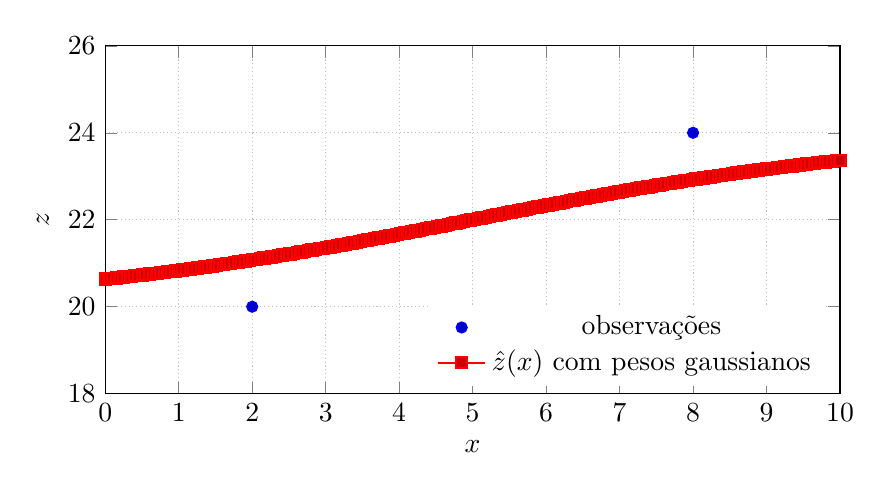
\begin{tikzpicture}
  \begin{axis}[
    width=0.9\linewidth, height=6cm,
    xlabel={$x$}, ylabel={$z$},
    xmin=0, xmax=10, ymin=18, ymax=26,
    grid=both, grid style={densely dotted},
    legend style={at={(0.98,0.02)},anchor=south east, draw=none}
  ]
    % Pontos observados (ex.: temperatura)
    \addplot+[only marks, mark=*] coordinates {(2,20) (8,24)}; \addlegendentry{observações}
    % Curva de interpolação ponderada (duas gaussianas normalizadas)
    \addplot+[domain=0:10, samples=200, thick]
      { (20*exp(-(x-2)^2/6^2) + 24*exp(-(x-8)^2/6^2)) / (exp(-(x-2)^2/6^2) + exp(-(x-8)^2/6^2)) };
    \addlegendentry{$\hat{z}(x)$ com pesos gaussianos}
  \end{axis}
\end{tikzpicture}
\caption{Interpolação 1D entre duas observações usando pesos gaussianos normalizados (raio efetivo $R\approx 6$). A estimativa transita suavemente entre os valores observados.}
\label{fig:interp-1d}
\end{figure}

\begin{figure}[h!]
\centering
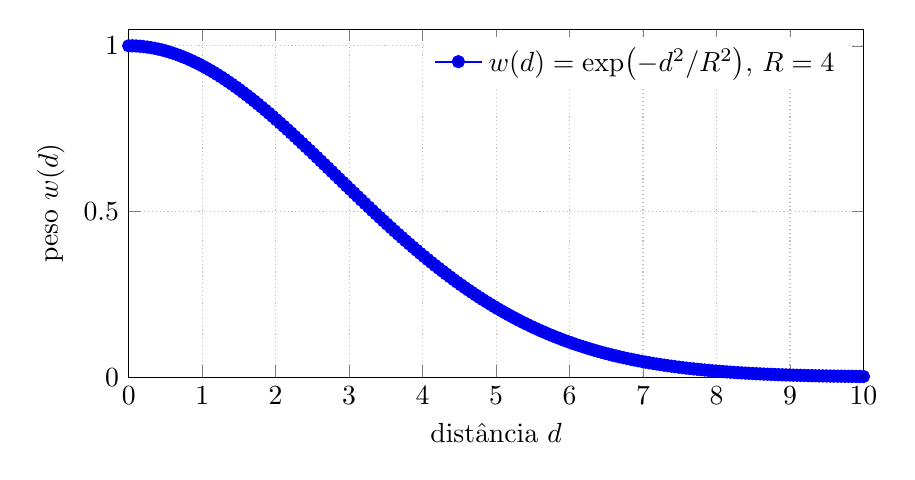
\begin{tikzpicture}
  \begin{axis}[
    width=0.9\linewidth, height=6cm,
    xlabel={distância $d$}, ylabel={peso $w(d)$},
    xmin=0, xmax=10, ymin=0, ymax=1.05,
    grid=both, grid style={densely dotted},
    legend style={at={(0.98,0.98)},anchor=north east, draw=none}
  ]
    \addplot+[domain=0:10, samples=200, thick]
      { exp(- (x^2) / 4^2) };
    \addlegendentry{$w(d)=\exp\!\left(-d^2/R^2\right)$, $R=4$}
  \end{axis}
\end{tikzpicture}
\caption{Função de peso gaussiana típica utilizada em análises espaciais: o peso decai rapidamente com a distância em relação ao raio $R$.}
\label{fig:peso-distancia}
\end{figure}

%---------------------------------------------------------
\section{Síntese}
A interpolação fornece a intuição: estimar nos vazios combinando vizinhança e suavidade. A AD amplia essa ideia ao incluir \emph{conhecimento de erro} --- tanto do modelo quanto das observações --- e formular a estimativa como uma \emph{combinação ótima}. Nos próximos capítulos, formalizaremos essa transição: dos ajustes (mínimos quadrados) à análise objetiva e, então, aos métodos modernos (VAR, EnKF e Kalman) que compõem o arsenal atual da assimilação de dados.

% Fim do Capítulo 1
